\chapter{Knihovna pro navrhování konstrukcí podle Eurokódů}

Knihovna \texttt{desssign} byla vyvinuta s cílem usnadnit klasifikaci, třídění a generování zatěžovacích stavů podle požadavků Eurokódu. Eurokódy představují soubor evropských norem pro navrhování konstrukcí, které obsahují specifické požadavky na kombinace zatížení a jejich součinitele. Tato knihovna umožňuje automatizaci tohoto procesu.

Hlavním důvodem vzniku knihovny bylo zajistit, aby bylo možné automaticky generovat kombinace zatěžovacích stavů podle jejich charakteru a přiřazovat jednotlivým zatěžovacím stavům odpovídající součinitele, jak to vyžadují Eurokódy. Tento přístup umožňuje snadno a rychle vytvářet správné kombinace zatížení, které mohou být následně použity v knihovně \texttt{framesss} pro statické výpočty prutových konstrukcí.

Při návrhu knihovny pro analýzu konstrukcí \texttt{framesss} jsem chtěl zachovat její obecnost a flexibilitu, aniž by byla zatížena specifickými normami nebo jinými specifickými závislostmi. Cílem bylo vytvořit obecný program pro analýzu prutových konstrukcí, který by nebyl příliš komplikovaný a nebyl závislý na konkrétní normě. Knihovna \texttt{desssign} tedy vznikla jako doplněk k \texttt{framesss}, aby umožnila specifickou implementaci podle Eurokódů, aniž by zatěžovala základní knihovnu zbytečnými závislostmi.

Knihovna \texttt{desssign} se skládá z několika modulů, z nichž nejvýznamnější je modul \texttt{loads}. Tento modul obsahuje třídy a funkce potřebné pro definici a správu zatěžovacích stavů a jejich kombinací. Mezi hlavní třídy patří \texttt{DesignLoadCase}, \texttt{DesignLoadCaseCombination} a \texttt{DesignLoadCaseGroup}, které umožňují definici vztahů mezi jednotlivými zatěžovacími stavy. Dále je zde třída \texttt{CombinationsGenerator}, která generuje kombinace zatížení na základě zadaného mezního stavu, typu kombinace a klasifikaci zatěžovacích stavů.

Knihovna také obsahuje submodul pro generování zatížení sněhem a větrem pro jednoduché tvary střech.

V následujících částech této kapitoly se podrobněji podíváme na architekturu knihovny \texttt{desssign}, jednotlivé moduly a jejich funkce, a také na praktické použití této knihovny v kontextu navrhování konstrukcí podle Eurokódů.

Zdrojový kód \texttt{desssign} je veřejně dostupný na platformě GitHub na adrese \url{https://github.com/DanBeranek/desssign}. Dokumentace knihovny, která je k dispozici na adrese \url{https://danberanek.github.io/desssign/index.html}, poskytuje podrobné informace o funkcionalitě, implementaci a použití knihovny.

\section{Instalace}
Knihovna \texttt{desssign} je snadno instalovatelná pomocí \texttt{pip}. Pro instalaci knihovny \texttt{framesss} stačí spustit následující příkaz v terminálu:

\begin{verbatim}
pip install desssign
\end{verbatim}

Podrobný návod na instalaci knihovny v Python virtuálním prostředí lze nalézt v \autoref{sec:framesss_instalation}.

\section{Architektura knihovny}
Knihovna \texttt{desssign} je navržena jako modulární a rozšiřitelný systém, který umožňuje snadnou integraci nových funkcionalit. Hlavní moduly knihovny zahrnují modul \texttt{loads} a modul \texttt{wood}. Tato část kapitoly se zaměří na popis struktury knihovny a jednotlivých modulů.

\subsection{Struktura knihovny}
Knihovna \texttt{desssign} je organizována do následujících hlavních modulů
\begin{itemize}
    \item \textbf{loads}: Tento modul obsahuje třídy a funkce pro definici, správu a generování kombinací zatěžovacích stavů. Hlavní třídy zahrnují \texttt{DesignLoadCase}, \texttt{DesignLoadCaseCombination}, \texttt{DesignLoadCaseGroup} a \texttt{CombinationsGenerator}. Tento modul také obsahuje submodul pro generování zatížení sněhem a větrem pro jednoduché tvary střech.
    \item \textbf{wood}: Tento modul obsahuje funkce pro posouzení dřevěných konstrukcí podle \textit{ČSN EN 1995-1-1}. Přestože se jedná o důležitou součást knihovny, v této diplomové práci se zaměříme především na modul \texttt{loads}.
\end{itemize}

\subsubsection*{Modul \texttt{loads}}
Modul \texttt{loads} je klíčovou součástí knihovny \texttt{desssign} a je zodpovědný za
\begin{itemize}
    \item \textbf{Definic zatěžovacích stavů}:  Pomocí tříd \texttt{DesignLoadCase} a \texttt{DesignLoadCaseCombination}, které dědí vlastnosti tříd z knihovny \texttt{framesss}, lze definovat jednotlivé zatěžovací stavy a jejich kombinace.
    \item \textbf{Kategorizaci zatěžovacích stavů}: Třída \texttt{DesignLoadCaseGroup} umožňuje definovat vztahy mezi jednotlivými zatěžovacími stavy.
    \item \textbf{Generování kombinací zatížení}: Třída \texttt{CombinationsGenerator} umožňuje automatické generování kombinací zatížení na základě zadaných parametrů a kategorizaci zatěžovacích stavů.
\end{itemize}

Tento modul také zahrnuje submodul pro klimatická zatížení, který umožňuje generování hodnot zatížení sněhem na střeše podle kapitoly 5 v ČSN EN 1991-1-3 \cite{EN1991_1_3} a zatížení větrem pro obdélníkový tvar střech podle kapitoly 5 v ČSN EN 1991-1-4 \cite{EN1991_1_4}.

\begin{figure}[H]
    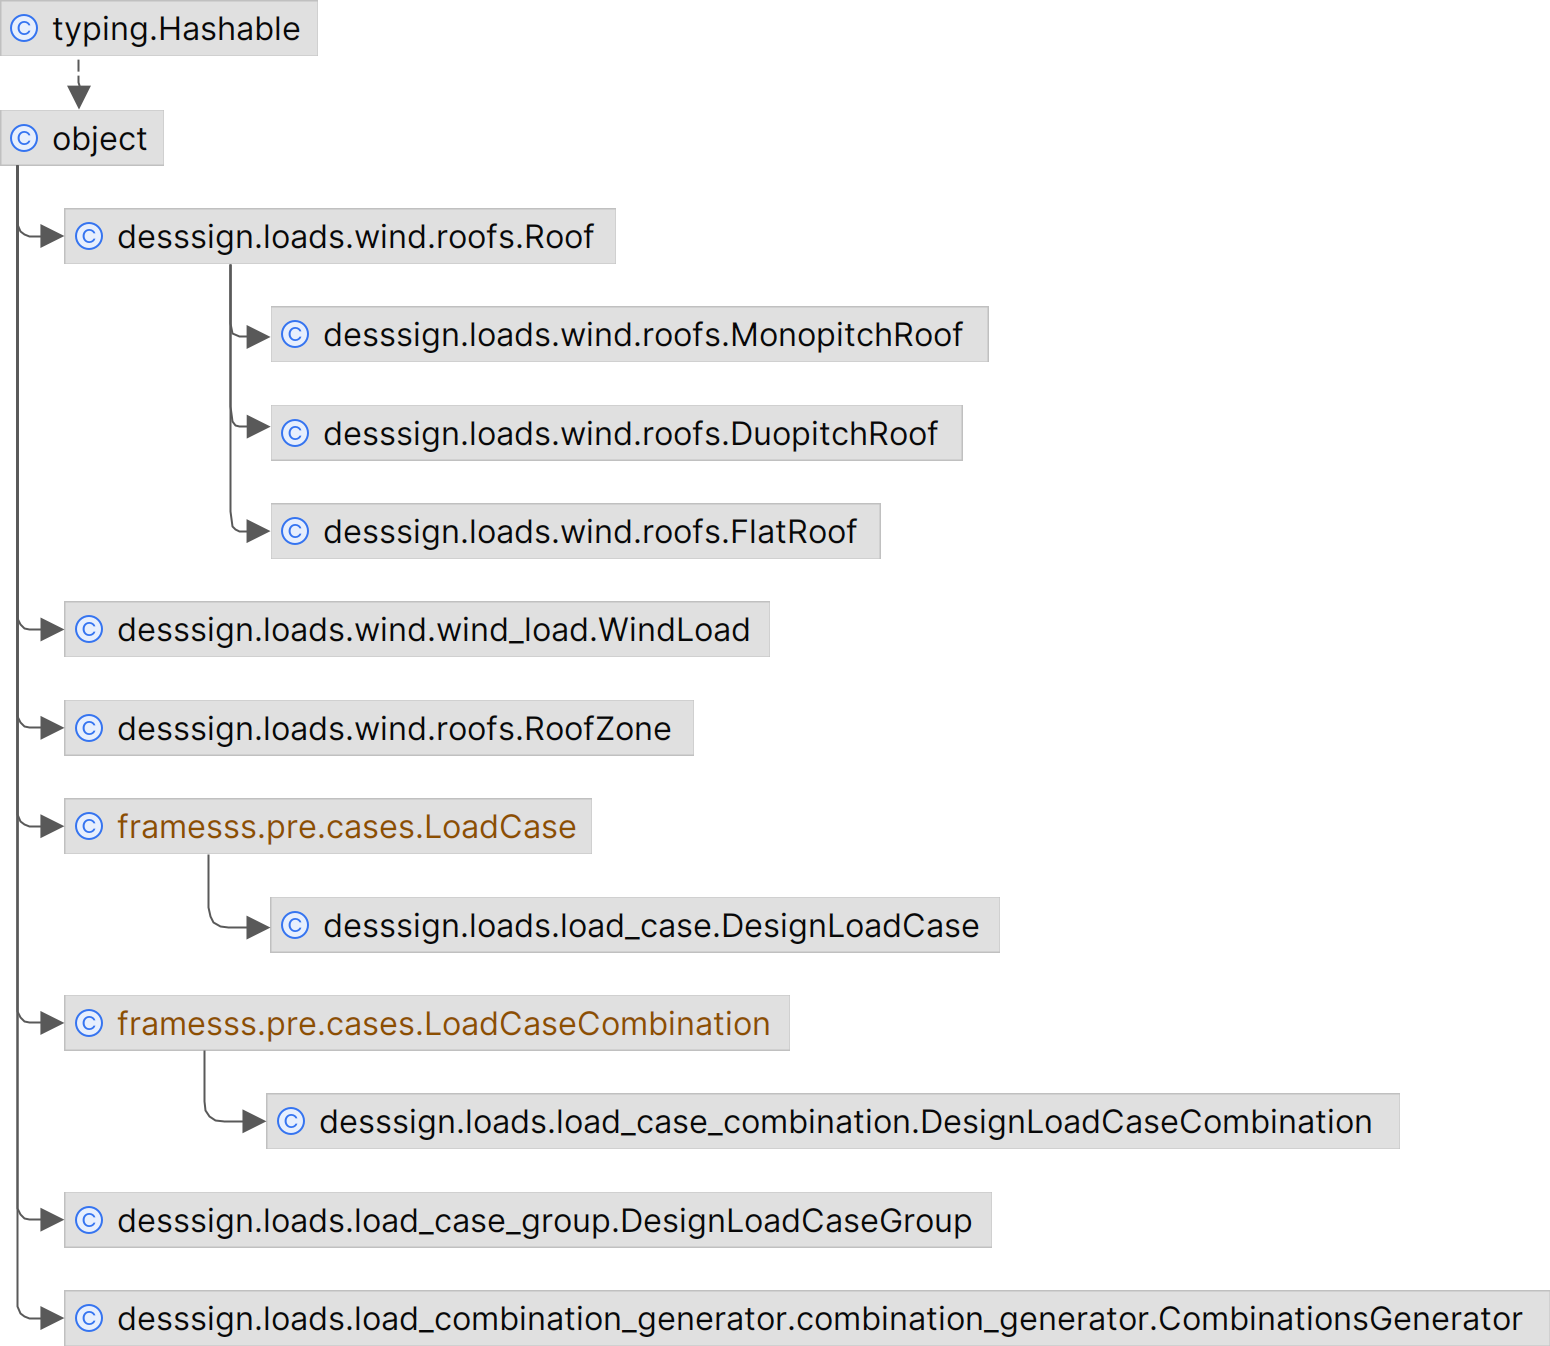
\includegraphics{assets/figures/desssign/loads_uml.png}
    \caption{Diagram modulu \texttt{loads}}
    \label{fig:modul_loads}
\end{figure}

\subsection{Integrace s knihovnou pro výpočty prutových konstrukcí}
Jednou z klíčových vlastností knihovny \texttt{desssign} je její schopnost generovat kombinace zatěžovacích stavů, které lze následně použít v knihovně \texttt{framesss} pro statické výpočty. Tímto způsobem knihovna \texttt{desssign} výrazně usnadňuje a automatizuje proces návrhu konstrukcí podle Eurokódů.

\subsubsection*{Třída \texttt{DesignLoadCase}}
Tato třída rozšiřuje třídu \texttt{LoadCase} z knihovny \texttt{framesss} a přidává specifické atributy, 
\begin{itemize}
    \item \texttt{load\_type}: typ zatížení, lze volit mezi stálým a užitným zatížením,
    \item \texttt{category}: kategorie zatížení podle ČSN EN 1991-1-1, kapitola 6.3.1.1 \cite{EN1991_1_1}, specifikuje se pouze pro užitné zatížení,
    \item \texttt{load\_duration\_class}: třída trvání zatížení podle ČSN EN 1995-1-1, tab. 2.1 \cite{EN1995_1_1}.
\end{itemize}

\begin{figure}[H]
    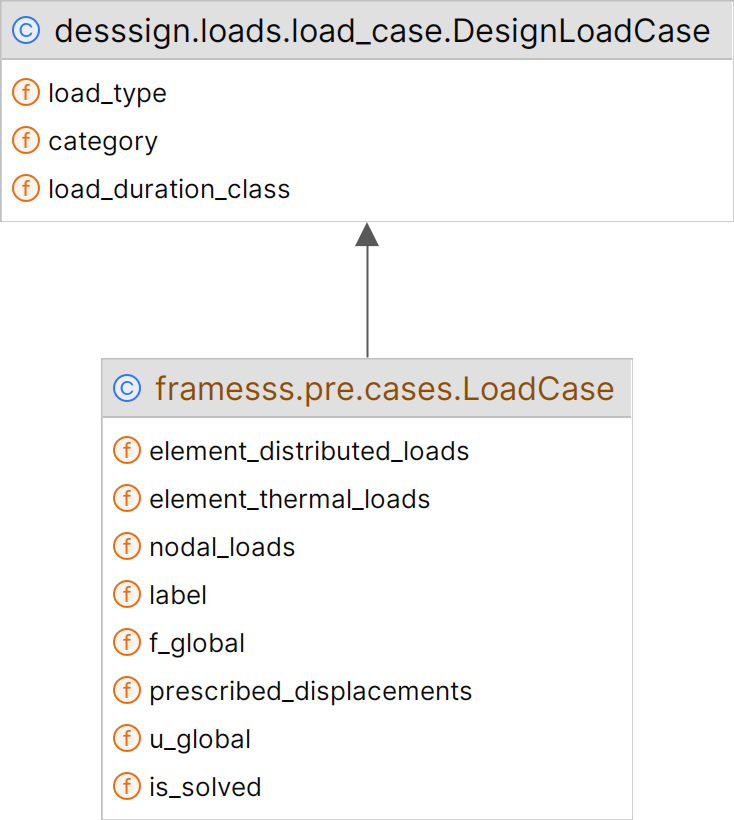
\includegraphics[height=8cm]{assets/figures/desssign/load_case.png}
    \caption{Diagram třídy \texttt{DesignLoadCase}}
    \label{fig:class_design_load_case}
\end{figure}

\subsubsection*{Třída \texttt{DesignLoadCaseCombination}}
Tato třída rozšiřuje třídu \texttt{LoadCaseCombination} z knihovny \texttt{framesss} a zahrnuje atributy
\begin{itemize}
    \item \texttt{permanent\_cases}: zatěžovací stavy pro stálé zatížení,
    \item \texttt{leading\_variable\_case}: zatěžovací stav pro hlavní proměnné zatížení,
    \item \texttt{other\_variable\_cases}: vedlejší proměnné zatěžovací stavy,
    \item \texttt{limit\_state}: mezní stav,
    \item \texttt{combination\_type}: typ kombinace,
    \item \texttt{alternative\_combination}: specifikátor použité rovnice, vyžadovaný pouze pro alternativní kombinace MSÚ, buď \texttt{'6.10a'}, nebo \texttt{'6.10b'}, 
    \item \texttt{combination\_key}: automaticky vygenerovaný kombinační klíč.
\end{itemize}

Podle zadaného mezního stavu a kombinace se jednotlivým zatěžovacím automaticky přiřadí kombinační součinitelé podle pravidel v ČSN EN 1990 \cite{EN1990}.

\begin{figure}[H]
    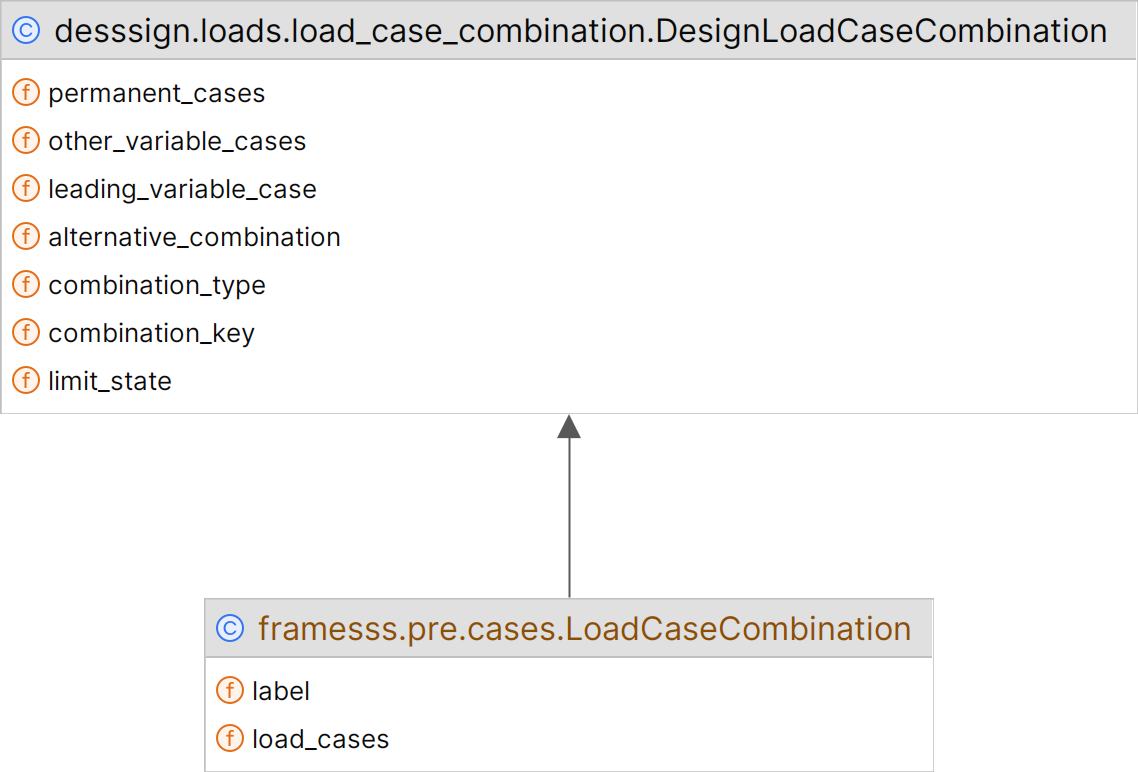
\includegraphics[height=8cm]{assets/figures/desssign/load_combinations.png}
    \caption{Diagram třídy \texttt{DesignLoadCaseComtination}}
    \label{fig:class_design_load_case_combination}
\end{figure}

\subsubsection*{Třída \texttt{DesignLoadCaseGroup}}
Třída \texttt{DesignLoadCaseGroup} umožňuje definovat vztahy mezi jednotlivými zatěžovacími stavy. Tato třída je klíčová pro správné generování kombinací zatěžovacích stavů.

Atributy:
\begin{itemize}
    \item \texttt{load\_case\_relation}: definuje vztah mezi zatěžovacími stavy,
    \begin{itemize}
        \item zatěžovací stavy působí vždy společně (např. stálá zatížení),
        \item zatěžovací stavy můžou a nemusí působit společně (např. užitná zatížení),
        \item zatížovací stavy nikdy nepůsobí společně.
    \end{itemize}
    \item \texttt{load\_cases}: zatěžovací stavy.
\end{itemize}

\begin{figure}[H]
    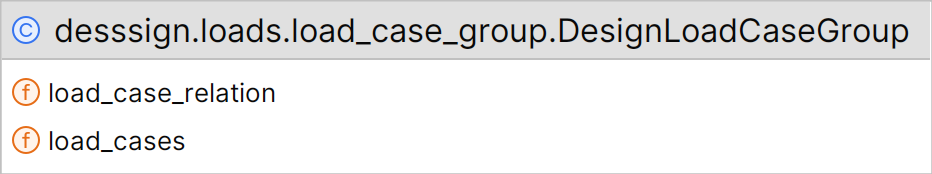
\includegraphics{assets/figures/desssign/design_load_case_group.png}
    \caption{Diagram třídy \texttt{DesignLoadCaseGroup}}
    \label{fig:class_design_load_case_group}
\end{figure}

\subsubsection*{Třída \texttt{CombinationsGenerator}}
Třída \texttt{CombinationsGenerator} je zodpovědná za generování kombinací zatížení na základě zadaného mezního stavu a typu kombinace.

Atributy:
\begin{itemize}
    \item \texttt{limit\_state}: typ mezního stavu (mezní stav únosnosti, mezni stav použitelnosti),
    \item \texttt{combination\_type}: typ kombinace zatížení (základní, alternativní, charakteristická, častá, kvazistálá)
\end{itemize}

Metody:
\begin{itemize}
    \item \texttt{generate\_combinations(load\_case\_groups)}: generuje kombinace zatížení na základě listu instancí \texttt{DesignLoadCaseGroup}.
\end{itemize}

Kombinace zatížení se generují podle vztahů uvedených v kapitole 6 ČSN EN 1990 \cite{EN1990},
\begin{itemize}
    \item mezní stavy únosnosti, kombinace pro trvalé a dočasné návrhové situace:
        \begin{itemize}
            \item základní kombinace zatížení podle vztahu 6.10,
            \begin{equation}
                \sum_{j \geq 1} \gamma_{G,j} G_{k,j} "+" \gamma_P P "+" \gamma_{Q,1} Q_{k,1} "+" \sum_{i > 1} \gamma_{Q,i} \psi_{0,i} Q_{k,i},
            \end{equation}
            \item alternativní kombinace zatížení podle vztahu 6.10a a 6.10b,
            \begin{subequations}
                \begin{equation}
                    \sum_{j \geq 1} \gamma_{G,j} G_{k,j} "+" \gamma_P P "+" \gamma_{Q,1} \psi_{0,1} Q_{k,1} "+" \sum_{i > 1} \gamma_{Q,i} \psi_{0,i} Q_{k,i},
                \end{equation}
                \begin{equation}
                    \sum_{j \geq 1} \xi_j \gamma_{G,j} G_{k,j} "+" \gamma_P P "+" \gamma_{Q,1} Q_{k,1} "+" \sum_{i > 1} \gamma_{Q,i} \psi_{0,i} Q_{k,i},
                \end{equation}
            \end{subequations}
        \end{itemize}
    \item mezní stavy použitelnosti,
    \begin{itemize}
        \item charakteristická kombinace zatížení podle vztahu 6.14b,
            \begin{equation}
                \sum_{j \geq 1} G_{k,j} "+" P "+" Q_{k,1} "+" \sum_{i > 1} \psi_{0,i} Q_{k,i},
            \end{equation}
        \item častá kombinace zatížení podle vztahu 6.15b,
            \begin{equation}
                \sum_{j \geq 1} G_{k,j} "+" P "+" \psi_{1,i} Q_{k,1} "+" \sum_{i > 1} \psi_{2,i} Q_{k,i},
            \end{equation}
        \item kvazistálou kombinaci zatížení podle vztahu 6.16b,
            \begin{equation}
                \sum_{j \geq 1} G_{k,j} "+" \sum_{i \geq 1} \psi_{2,i} Q_{k,i},
            \end{equation}
    \end{itemize}
\end{itemize}
kde $G$ označuje stálé zatížení, $Q$ proměnné zatížení, $Q_{1}$ označuje hlavní proměnné zatížení, $\gamma$ jsou dílčí součinitelé zatížení podle ČSN EN 1990, příloha A \cite{EN1990}, $\psi$ jsou součinitele pro proměnná zatížení podle ČSN EN 1990, příloha A \cite{EN1990} a $\xi$ je redukční součinitel pro stálé zatížení.

\section{Příklad použití}

Pro klasifikaci zatěžovacích jsou v knihovně vytvořeny \texttt{Enum}\footnote{\texttt{Enum} je speciální datový typ, který umožňuje definovat sadu pojmenovaných konstant.} třídy, které jasně stanovují způsob, jakým způsobem se mají zadávat parametry při vytváření nových instancí. Tyto \texttt{Enum} třídy zajišťují, že parametry jsou zadávány konzistentně a správně, což minimalizuje riziko chyb při definování zatěžovacích stavů.

Nejprve musíme do prostředí JupyterLab importovat všechny potřebné třídy a balíčky.
\begin{tcolorbox}[breakable, size=fbox, boxrule=1pt, pad at break*=1mm,colback=cellbackground, colframe=cellborder]
    \prompt{In}{incolor}{1}{\boxspacing}
    \begin{Verbatim}[commandchars=\\\{\}]
    \PY{k+kn}{from} \PY{n+nn}{desssign}\PY{n+nn}{.}\PY{n+nn}{loads}\PY{n+nn}{.}\PY{n+nn}{enums} \PY{k+kn}{import} \PY{n}{LoadType}
    \PY{k+kn}{from} \PY{n+nn}{desssign}\PY{n+nn}{.}\PY{n+nn}{loads}\PY{n+nn}{.}\PY{n+nn}{enums} \PY{k+kn}{import} \PY{n}{LimitState}
    \PY{k+kn}{from} \PY{n+nn}{desssign}\PY{n+nn}{.}\PY{n+nn}{loads}\PY{n+nn}{.}\PY{n+nn}{enums} \PY{k+kn}{import} \PY{n}{VariableCategory} \PY{k}{as} \PY{n}{cat}
    \PY{k+kn}{from} \PY{n+nn}{desssign}\PY{n+nn}{.}\PY{n+nn}{loads}\PY{n+nn}{.}\PY{n+nn}{enums} \PY{k+kn}{import} \PY{n}{ULSCombination} \PY{k}{as} \PY{n}{uls}
    \PY{k+kn}{from} \PY{n+nn}{desssign}\PY{n+nn}{.}\PY{n+nn}{loads}\PY{n+nn}{.}\PY{n+nn}{enums} \PY{k+kn}{import} \PY{n}{SLSCombination} \PY{k}{as} \PY{n}{sls}
    \PY{k+kn}{from} \PY{n+nn}{desssign}\PY{n+nn}{.}\PY{n+nn}{loads}\PY{n+nn}{.}\PY{n+nn}{enums} \PY{k+kn}{import} \PY{n}{ULSAlternativeCombination} \PY{k}{as} \PY{n}{alt}
    \PY{k+kn}{from} \PY{n+nn}{desssign}\PY{n+nn}{.}\PY{n+nn}{loads}\PY{n+nn}{.}\PY{n+nn}{enums} \PY{k+kn}{import} \PY{n}{LoadCaseRelation} \PY{k}{as} \PY{n}{rel}
    
    \PY{k+kn}{from} \PY{n+nn}{desssign}\PY{n+nn}{.}\PY{n+nn}{loads}\PY{n+nn}{.}\PY{n+nn}{load\PYZus{}case} \PY{k+kn}{import} \PY{n}{DesignLoadCase}
    \PY{k+kn}{from} \PY{n+nn}{desssign}\PY{n+nn}{.}\PY{n+nn}{loads}\PY{n+nn}{.}\PY{n+nn}{load\PYZus{}case\PYZus{}group} \PY{k+kn}{import} \PY{n}{DesignLoadCaseGroup}
    \PY{k+kn}{from} \PY{n+nn}{desssign}\PY{n+nn}{.}\PY{n+nn}{loads}\PY{n+nn}{.}\PY{n+nn}{load\PYZus{}combination\PYZus{}generator}\PY{n+nn}{.}\PY{n+nn}{combination\PYZus{}generator} \PY{k+kn}{import} \PY{n}{CombinationsGenerator}
    \end{Verbatim}
    \end{tcolorbox}

Vytvoříme 5 instancí typu \texttt{DesignLoadCase}, dva zatěžovací stavy pro stálé zatížení (\texttt{G1, G2}), jeden zatěžovací stav pro užitné zatížení kategorie A (\texttt{Q3}) a dva zatěžovací stavy pro zatížení sněhem (\texttt{S4, S5}).
        \begin{tcolorbox}[breakable, size=fbox, boxrule=1pt, pad at break*=1mm,colback=cellbackground, colframe=cellborder]
    \prompt{In}{incolor}{2}{\boxspacing}
    \begin{Verbatim}[commandchars=\\\{\}]
    \PY{n}{G1} \PY{o}{=} \PY{n}{DesignLoadCase}\PY{p}{(}
        \PY{n}{label}\PY{o}{=}\PY{l+s+s2}{\PYZdq{}}\PY{l+s+s2}{G1}\PY{l+s+s2}{\PYZdq{}}\PY{p}{,}
        \PY{n}{load\PYZus{}type}\PY{o}{=}\PY{n}{LoadType}\PY{o}{.}\PY{n}{PERMANENT}\PY{p}{,}
    \PY{p}{)}
    
    \PY{n}{G2} \PY{o}{=} \PY{n}{DesignLoadCase}\PY{p}{(}
        \PY{n}{label}\PY{o}{=}\PY{l+s+s2}{\PYZdq{}}\PY{l+s+s2}{G2}\PY{l+s+s2}{\PYZdq{}}\PY{p}{,}
        \PY{n}{load\PYZus{}type}\PY{o}{=}\PY{n}{LoadType}\PY{o}{.}\PY{n}{PERMANENT}\PY{p}{,}
    \PY{p}{)}
    
    \PY{n}{Q3} \PY{o}{=} \PY{n}{DesignLoadCase}\PY{p}{(}
        \PY{n}{label}\PY{o}{=}\PY{l+s+s2}{\PYZdq{}}\PY{l+s+s2}{Q3}\PY{l+s+s2}{\PYZdq{}}\PY{p}{,}
        \PY{n}{load\PYZus{}type}\PY{o}{=}\PY{n}{LoadType}\PY{o}{.}\PY{n}{VARIABLE}\PY{p}{,}
        \PY{n}{category}\PY{o}{=}\PY{n}{cat}\PY{o}{.}\PY{n}{A}\PY{p}{,}
    \PY{p}{)}
    
    \PY{n}{S4} \PY{o}{=} \PY{n}{DesignLoadCase}\PY{p}{(}
        \PY{n}{label}\PY{o}{=}\PY{l+s+s2}{\PYZdq{}}\PY{l+s+s2}{S4}\PY{l+s+s2}{\PYZdq{}}\PY{p}{,}
        \PY{n}{load\PYZus{}type}\PY{o}{=}\PY{n}{LoadType}\PY{o}{.}\PY{n}{VARIABLE}\PY{p}{,}
        \PY{n}{category}\PY{o}{=}\PY{n}{cat}\PY{o}{.}\PY{n}{SNOW\PYZus{}BELLOW\PYZus{}1000\PYZus{}M}\PY{p}{,}
    \PY{p}{)}
    
    
    \PY{n}{S5} \PY{o}{=} \PY{n}{DesignLoadCase}\PY{p}{(}
        \PY{n}{label}\PY{o}{=}\PY{l+s+s2}{\PYZdq{}}\PY{l+s+s2}{S5}\PY{l+s+s2}{\PYZdq{}}\PY{p}{,}
        \PY{n}{load\PYZus{}type}\PY{o}{=}\PY{n}{LoadType}\PY{o}{.}\PY{n}{VARIABLE}\PY{p}{,}
        \PY{n}{category}\PY{o}{=}\PY{n}{cat}\PY{o}{.}\PY{n}{SNOW\PYZus{}BELLOW\PYZus{}1000\PYZus{}M}\PY{p}{,}
    \PY{p}{)}
    \end{Verbatim}
    \end{tcolorbox}

    Vytvoříme skupiny zatížení, zatěžovací stavy ve skupině pro stálé zatížení, \texttt{LG\_permanent}, působí v každé kombinaci dohromady. Skupina zatížení pro užitné zatížení, \texttt{LG\_imposed}, je typu \texttt{STANDARD}. Zatěžovací stavy ve skupině pro zatížení sněhem, \texttt{LG\_snow}, nepůsobí v žádné kombinaci společně.
        \begin{tcolorbox}[breakable, size=fbox, boxrule=1pt, pad at break*=1mm,colback=cellbackground, colframe=cellborder]
    \prompt{In}{incolor}{3}{\boxspacing}
    \begin{Verbatim}[commandchars=\\\{\}]
    \PY{n}{LG\PYZus{}permanent} \PY{o}{=} \PY{n}{DesignLoadCaseGroup}\PY{p}{(}
        \PY{n}{load\PYZus{}cases}\PY{o}{=}\PY{p}{[}\PY{n}{G1}\PY{p}{,} \PY{n}{G2}\PY{p}{]}\PY{p}{,}
        \PY{n}{load\PYZus{}case\PYZus{}relation}\PY{o}{=}\PY{n}{rel}\PY{o}{.}\PY{n}{TOGETHER}\PY{p}{,}
    \PY{p}{)}
    
    \PY{n}{LG\PYZus{}imposed} \PY{o}{=} \PY{n}{DesignLoadCaseGroup}\PY{p}{(}
        \PY{n}{load\PYZus{}cases}\PY{o}{=}\PY{p}{[}\PY{n}{Q3}\PY{p}{]}\PY{p}{,}
        \PY{n}{load\PYZus{}case\PYZus{}relation}\PY{o}{=}\PY{n}{rel}\PY{o}{.}\PY{n}{STANDARD}\PY{p}{,}
    \PY{p}{)}
    
    \PY{n}{LG\PYZus{}snow} \PY{o}{=} \PY{n}{DesignLoadCaseGroup}\PY{p}{(}
        \PY{n}{load\PYZus{}cases}\PY{o}{=}\PY{p}{[}\PY{n}{S4}\PY{p}{,} \PY{n}{S5}\PY{p}{]}\PY{p}{,}
        \PY{n}{load\PYZus{}case\PYZus{}relation}\PY{o}{=}\PY{n}{rel}\PY{o}{.}\PY{n}{EXCLUSIVE}\PY{p}{,}
    \PY{p}{)}
    \end{Verbatim}
    \end{tcolorbox}
    
    Inicializujeme generátor pro generování základních kombinací pro mezní stav únosnosti.
        \begin{tcolorbox}[breakable, size=fbox, boxrule=1pt, pad at break*=1mm,colback=cellbackground, colframe=cellborder]
    \prompt{In}{incolor}{4}{\boxspacing}
    \begin{Verbatim}[commandchars=\\\{\}]
    \PY{n}{ULS\PYZus{}basic\PYZus{}generator} \PY{o}{=} \PY{n}{CombinationsGenerator}\PY{p}{(}
        \PY{n}{limit\PYZus{}state}\PY{o}{=}\PY{n}{LimitState}\PY{o}{.}\PY{n}{ULS}\PY{p}{,}
        \PY{n}{combination\PYZus{}type}\PY{o}{=}\PY{n}{uls}\PY{o}{.}\PY{n}{BASIC}
    \PY{p}{)}
    \end{Verbatim}
    \end{tcolorbox}
    
Pomocí metody \texttt{generate\_combinations()} vygenerujeme kombinace a uložíme je do proměnné \texttt{combinations}.
        \begin{tcolorbox}[breakable, size=fbox, boxrule=1pt, pad at break*=1mm,colback=cellbackground, colframe=cellborder]
    \prompt{In}{incolor}{5}{\boxspacing}
    \begin{Verbatim}[commandchars=\\\{\}]
    \PY{n}{combinations} \PY{o}{=} \PY{n}{ULS\PYZus{}basic\PYZus{}generator}\PY{o}{.}\PY{n}{generate\PYZus{}combinations}\PY{p}{(}
        \PY{p}{[}\PY{n}{LG\PYZus{}permanent}\PY{p}{,} \PY{n}{LG\PYZus{}imposed}\PY{p}{,} \PY{n}{LG\PYZus{}snow}\PY{p}{]}
    \PY{p}{)}
    \end{Verbatim}
    \end{tcolorbox}

Vypíšeme automaticky vygenerovaný název a klíč kombinace, který obsahuje jednotlivé součinitele určené podle ČSN EN 1990.
        \begin{tcolorbox}[breakable, size=fbox, boxrule=1pt, pad at break*=1mm,colback=cellbackground, colframe=cellborder]
    \prompt{In}{incolor}{6}{\boxspacing}
    \begin{Verbatim}[commandchars=\\\{\}]
    \PY{k}{for} \PY{n}{combination} \PY{o+ow}{in} \PY{n}{combinations}\PY{p}{:}
        \PY{n+nb}{print}\PY{p}{(}\PY{l+s+sa}{f}\PY{l+s+s2}{\PYZdq{}}\PY{l+s+s2}{Kombinace: }\PY{l+s+si}{\PYZob{}}\PY{n}{combination}\PY{o}{.}\PY{n}{label}\PY{l+s+si}{\PYZcb{}}\PY{l+s+s2}{\PYZdq{}}\PY{p}{)}
        \PY{n+nb}{print}\PY{p}{(}\PY{l+s+sa}{f}\PY{l+s+s2}{\PYZdq{}}\PY{l+s+s2}{Klíč: }\PY{l+s+si}{\PYZob{}}\PY{n}{combination}\PY{o}{.}\PY{n}{combination\PYZus{}key}\PY{l+s+si}{\PYZcb{}}\PY{l+s+se}{\PYZbs{}n}\PY{l+s+s2}{\PYZdq{}}\PY{p}{)}
    \end{Verbatim}
    \end{tcolorbox}
    
        \begin{Verbatim}[commandchars=\\\{\}]
    Kombinace: ULS-basic(1)
    Klíč: 1.35*G1+1.35*G2
    
    Kombinace: ULS-basic(2)
    Klíč: 1.35*G1+1.35*G2+1.5*S4
    
    Kombinace: ULS-basic(3)
    Klíč: 1.35*G1+1.35*G2+1.5*S5
    
    Kombinace: ULS-basic(4)
    Klíč: 1.35*G1+1.35*G2+1.5*Q3
    
    Kombinace: ULS-basic(5)
    Klíč: 1.35*G1+1.35*G2+1.5*Q3+1.5*0.5*S4
    
    Kombinace: ULS-basic(6)
    Klíč: 1.35*G1+1.35*G2+1.5*S4+1.5*0.7*Q3
    
    Kombinace: ULS-basic(7)
    Klíč: 1.35*G1+1.35*G2+1.5*Q3+1.5*0.5*S5
    
    Kombinace: ULS-basic(8)
    Klíč: 1.35*G1+1.35*G2+1.5*S5+1.5*0.7*Q3
    
        \end{Verbatim}
    
    Pro ilustraci dále vygenerujeme charakteristické kombinace zatížení pro mezní stav použitelnosti.
        \begin{tcolorbox}[breakable, size=fbox, boxrule=1pt, pad at break*=1mm,colback=cellbackground, colframe=cellborder]
    \prompt{In}{incolor}{7}{\boxspacing}
    \begin{Verbatim}[commandchars=\\\{\}]
    \PY{n}{SLS\PYZus{}char\PYZus{}generator} \PY{o}{=} \PY{n}{CombinationsGenerator}\PY{p}{(}
        \PY{n}{limit\PYZus{}state}\PY{o}{=}\PY{n}{LimitState}\PY{o}{.}\PY{n}{SLS}\PY{p}{,}
        \PY{n}{combination\PYZus{}type}\PY{o}{=}\PY{n}{sls}\PY{o}{.}\PY{n}{CHARACTERISTIC}
    \PY{p}{)}
    \end{Verbatim}
    \end{tcolorbox}
    
        \begin{tcolorbox}[breakable, size=fbox, boxrule=1pt, pad at break*=1mm,colback=cellbackground, colframe=cellborder]
    \prompt{In}{incolor}{8}{\boxspacing}
    \begin{Verbatim}[commandchars=\\\{\}]
    \PY{n}{combinations} \PY{o}{=} \PY{n}{SLS\PYZus{}char\PYZus{}generator}\PY{o}{.}\PY{n}{generate\PYZus{}combinations}\PY{p}{(}
        \PY{p}{[}\PY{n}{LG\PYZus{}permanent}\PY{p}{,} \PY{n}{LG\PYZus{}imposed}\PY{p}{,} \PY{n}{LG\PYZus{}snow}\PY{p}{]}
    \PY{p}{)}
    \end{Verbatim}
    \end{tcolorbox}
    
        \begin{tcolorbox}[breakable, size=fbox, boxrule=1pt, pad at break*=1mm,colback=cellbackground, colframe=cellborder]
    \prompt{In}{incolor}{9}{\boxspacing}
    \begin{Verbatim}[commandchars=\\\{\}]
    \PY{k}{for} \PY{n}{combination} \PY{o+ow}{in} \PY{n}{combinations}\PY{p}{:}
        \PY{n+nb}{print}\PY{p}{(}\PY{l+s+sa}{f}\PY{l+s+s2}{\PYZdq{}}\PY{l+s+s2}{Kombinace: }\PY{l+s+si}{\PYZob{}}\PY{n}{combination}\PY{o}{.}\PY{n}{label}\PY{l+s+si}{\PYZcb{}}\PY{l+s+s2}{\PYZdq{}}\PY{p}{)}
        \PY{n+nb}{print}\PY{p}{(}\PY{l+s+sa}{f}\PY{l+s+s2}{\PYZdq{}}\PY{l+s+s2}{Klíč: }\PY{l+s+si}{\PYZob{}}\PY{n}{combination}\PY{o}{.}\PY{n}{combination\PYZus{}key}\PY{l+s+si}{\PYZcb{}}\PY{l+s+se}{\PYZbs{}n}\PY{l+s+s2}{\PYZdq{}}\PY{p}{)}
    \end{Verbatim}
    \end{tcolorbox}
    
        \begin{Verbatim}[commandchars=\\\{\}]
    Kombinace: SLS-characteristic(1)
    Klíč: G1+G2
    
    Kombinace: SLS-characteristic(2)
    Klíč: G1+G2+S4
    
    Kombinace: SLS-characteristic(3)
    Klíč: G1+G2+S5
    
    Kombinace: SLS-characteristic(4)
    Klíč: G1+G2+Q3
    
    Kombinace: SLS-characteristic(5)
    Klíč: G1+G2+Q3+0.5*S4
    
    Kombinace: SLS-characteristic(6)
    Klíč: G1+G2+S4+0.7*Q3
    
    Kombinace: SLS-characteristic(7)
    Klíč: G1+G2+Q3+0.5*S5
    
    Kombinace: SLS-characteristic(8)
    Klíč: G1+G2+S5+0.7*Q3
    
        \end{Verbatim}
    
    Při generování alternativních kombinací pro mezní stav únosnosti se vygeneruje dvojnásobný počet kombinací, vždy jedna kombinace pro redukované hlavní proměnné zatížení a druhá kombinace pro redukované stálé zatížení.
        \begin{tcolorbox}[breakable, size=fbox, boxrule=1pt, pad at break*=1mm,colback=cellbackground, colframe=cellborder]
    \prompt{In}{incolor}{10}{\boxspacing}
    \begin{Verbatim}[commandchars=\\\{\}]
    \PY{n}{ULS\PYZus{}alt\PYZus{}generator} \PY{o}{=} \PY{n}{CombinationsGenerator}\PY{p}{(}
        \PY{n}{limit\PYZus{}state}\PY{o}{=}\PY{n}{LimitState}\PY{o}{.}\PY{n}{ULS}\PY{p}{,}
        \PY{n}{combination\PYZus{}type}\PY{o}{=}\PY{n}{uls}\PY{o}{.}\PY{n}{ALTERNATIVE}
    \PY{p}{)}
    \end{Verbatim}
    \end{tcolorbox}
    
        \begin{tcolorbox}[breakable, size=fbox, boxrule=1pt, pad at break*=1mm,colback=cellbackground, colframe=cellborder]
    \prompt{In}{incolor}{11}{\boxspacing}
    \begin{Verbatim}[commandchars=\\\{\}]
    \PY{n}{combinations} \PY{o}{=} \PY{n}{ULS\PYZus{}alt\PYZus{}generator}\PY{o}{.}\PY{n}{generate\PYZus{}combinations}\PY{p}{(}
        \PY{p}{[}\PY{n}{LG\PYZus{}permanent}\PY{p}{,} \PY{n}{LG\PYZus{}imposed}\PY{p}{,} \PY{n}{LG\PYZus{}snow}\PY{p}{]}
    \PY{p}{)}
    \end{Verbatim}
    \end{tcolorbox}
    
        \begin{tcolorbox}[breakable, size=fbox, boxrule=1pt, pad at break*=1mm,colback=cellbackground, colframe=cellborder]
    \prompt{In}{incolor}{12}{\boxspacing}
    \begin{Verbatim}[commandchars=\\\{\}]
    \PY{k}{for} \PY{n}{combination} \PY{o+ow}{in} \PY{n}{combinations}\PY{p}{:}
        \PY{n+nb}{print}\PY{p}{(}\PY{l+s+sa}{f}\PY{l+s+s2}{\PYZdq{}}\PY{l+s+s2}{Kombinace: }\PY{l+s+si}{\PYZob{}}\PY{n}{combination}\PY{o}{.}\PY{n}{label}\PY{l+s+si}{\PYZcb{}}\PY{l+s+s2}{\PYZdq{}}\PY{p}{)}
        \PY{n+nb}{print}\PY{p}{(}\PY{l+s+sa}{f}\PY{l+s+s2}{\PYZdq{}}\PY{l+s+s2}{Klíč: }\PY{l+s+si}{\PYZob{}}\PY{n}{combination}\PY{o}{.}\PY{n}{combination\PYZus{}key}\PY{l+s+si}{\PYZcb{}}\PY{l+s+se}{\PYZbs{}n}\PY{l+s+s2}{\PYZdq{}}\PY{p}{)}
    \end{Verbatim}
    \end{tcolorbox}
    
        \begin{Verbatim}[commandchars=\\\{\}]
    Kombinace: ULS-alternative(1a)
    Klíč: 1.35*G1+1.35*G2
    
    Kombinace: ULS-alternative(1b)
    Klíč: 0.85*1.35*G1+0.85*1.35*G2
    
    Kombinace: ULS-alternative(2a)
    Klíč: 1.35*G1+1.35*G2+1.5*0.5*S4
    
    Kombinace: ULS-alternative(2b)
    Klíč: 0.85*1.35*G1+0.85*1.35*G2+1.5*S4
    
    Kombinace: ULS-alternative(3a)
    Klíč: 1.35*G1+1.35*G2+1.5*0.5*S5
    
    Kombinace: ULS-alternative(3b)
    Klíč: 0.85*1.35*G1+0.85*1.35*G2+1.5*S5
    
    Kombinace: ULS-alternative(4a)
    Klíč: 1.35*G1+1.35*G2+1.5*0.7*Q3
    
    Kombinace: ULS-alternative(4b)
    Klíč: 0.85*1.35*G1+0.85*1.35*G2+1.5*Q3
    
    Kombinace: ULS-alternative(5a)
    Klíč: 1.35*G1+1.35*G2+1.5*0.7*Q3+1.5*0.5*S4
    
    Kombinace: ULS-alternative(5b)
    Klíč: 0.85*1.35*G1+0.85*1.35*G2+1.5*Q3+1.5*0.5*S4
    
    Kombinace: ULS-alternative(6a)
    Klíč: 1.35*G1+1.35*G2+1.5*0.5*S4+1.5*0.7*Q3
    
    Kombinace: ULS-alternative(6b)
    Klíč: 0.85*1.35*G1+0.85*1.35*G2+1.5*S4+1.5*0.7*Q3
    
    Kombinace: ULS-alternative(7a)
    Klíč: 1.35*G1+1.35*G2+1.5*0.7*Q3+1.5*0.5*S5
    
    Kombinace: ULS-alternative(7b)
    Klíč: 0.85*1.35*G1+0.85*1.35*G2+1.5*Q3+1.5*0.5*S5
    
    Kombinace: ULS-alternative(8a)
    Klíč: 1.35*G1+1.35*G2+1.5*0.5*S5+1.5*0.7*Q3
    
    Kombinace: ULS-alternative(8b)
    Klíč: 0.85*1.35*G1+0.85*1.35*G2+1.5*S5+1.5*0.7*Q3
    
        \end{Verbatim}

Takto vygenerované kombinace je možné použít v kombinaci s knihovnou \texttt{framesss}.